\chapter{Optical Lattices}
The dipole potential (equation \ref{dipolepot}) scales with the intensity of the laser. Thus, superimposing laser beams allows for creating a multitude of different potentials. A simple standing wave will lead to an array of potential wells
\begin{equation}
	V(z) = - V_0 \cos^2{k z } \; ,
	\label{standwave}
\end{equation}
 where $V_0 = | \frac{3 \pi c^2}{2 \omega_{0}^3} \frac{\Gamma}{\Delta} 4 I_0 |$. By adding beams from multiple directions the resulting wells form a lattice allowing one to mimic the physics of a solid state system. 

\section{Band Structure}
Consider a periodic potential as described by equation \ref{standwave}. \textit{Bloch's Theorem} states that energy eigenstates of a periodic potential with lattice vector $\boldsymbol{R}$ and quasi-momentum $q$ can be written as Bloch waves, which takes the form
\begin{equation}
	\psi_{\boldsymbol{q}}^{(n)}(\boldsymbol{r}) = e^{i \boldsymbol{q} \boldsymbol{r}} u^{(n)}(\boldsymbol{r}) \; ,
\end{equation}
which is a plane wave modulated by a function with the same periodicity as the potential $u^{(n)}(\boldsymbol{r}) = u^{(n)}(\boldsymbol{r} + \boldsymbol{R})$. Furthermore, the Bloch waves are periodic in reciprocal space, such that $\psi_{\boldsymbol{q}}^{(n)}(\boldsymbol{r}) = \psi_{\boldsymbol{q} + \boldsymbol{G}}^{(n)}(\boldsymbol{r})$, where $\boldsymbol{G}$ is a reciprocal lattice vector. \cite{kittel} \\
This leads to an energy spectrum in the shape of bands with the periodicity of the first \textit{Brillouin Zone}. Bands are denoted by the band index $n$, and their shape is determined by both the shape and the depth of the potential.\\
The potential depth is often denoted in units of the recoil energy $E_r = \frac{\hbar ^2 k^2}{2 m}$, where $m$ is the mass of the particle and $k$ the photon wave number of the light forming the optical lattice. For $V_0 = 0$ the particles are free, hence the bands will be parabolic. Meanwhile, for $V_0 \rightarrow \infty$ the wells become infinitely deep and thus disconnected, causing them to act like harmonic oscillators. Hence, the bands will appear flat with equal spacing. This can be seen in figure \ref{fig:blochbands}.
\begin{figure}[!h]
	\centering
	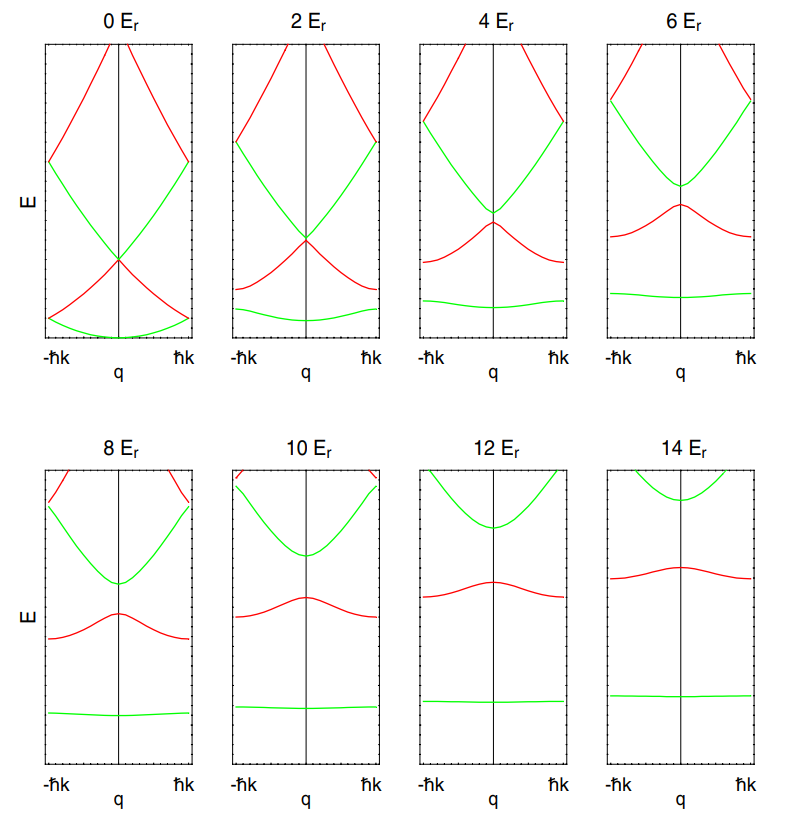
\includegraphics[width=0.9\columnwidth]{Figures/blochbands.png} 
	\caption{\textit{Band structure of an optical lattice: Energy of the Bloch state 		versus quasi momentum q in the first Brillouin zone, plotted for different 				lattice depths between 0 and 14 $E_r$. For deep lattices the lowest band 				becomes flat and the width of the first band gap corresponds to the level 				spacing $\hbar \omega$ on each lattice site. The figure and caption are 				adopted from \cite{greiner}.}}
	\label{fig:blochbands} 
\end{figure}


\section{Localized States}
The region $5 E_r \leq V_0 \leq 8 E_r$ is called the \textit{tight binding limit}, where interactions between wells almost purely are next-neighbour interactions. In this limit the wavefunctions are well localized prompting the use of a basis in real space. Wannier functions constitute a set of orthonormal functions given by
\begin{equation}
	w^{(n)}(\boldsymbol{r}) = \frac{1}{\sqrt{N_L}} \sum_{q} e^{ -i \boldsymbol{q} \boldsymbol{r} } \psi_{\boldsymbol{q}}^{(n)}(\boldsymbol{r}) \; ,
\end{equation} 
where $N_L$ is the number of primitive cells of the lattice. The localized Wannier functions are lattice periodic $w^{(n)}(\boldsymbol{r}) = w^{(n)}(\boldsymbol{r} + \boldsymbol{R})$ consists of a Fourier transform of de-localized Bloch waves. \cite{manybodyBloch}